%
\chapter{Planning, Control \& State Estimation}%
\label{chap:planningcontrol}
In this chapter the most common planning, control and state estimation strategies are pointed out and reviewed. As mentioned before, publications that regard the humanoid robots in use at IHMC, get special consideration.

\section{Planning}
In robotics, the planning problem can be described with a desired final goal of the motion, constraints on the path itself as terrain where collision needs to be avoided and constraints on the capabilities of the system as kinematic limits and actuation limits. As the dynamics of a humanoid robot are complex and underactuated, there exist numerous way to generate a walking plan. This typically ranges from reactive stepping and tracking a desired velocity to precise foot placements. In this section common planning strategies are described.

\subsection{Footstep planning}
While not all bipedal robots require a footstep plan to walk, most humanoids do. A footstep plan is a sequence of foothold references on the ground. Those can be computed either offline or online. Offline, either an autonomous planner can make a plan, or a robot operator can define desired footsteps manually. Online the robot in some cases can re-plan to avoid collision or adjust a footstep to use for stabilization. In \cite{chestnutt2005footstep} is described how an online plan can be generated as an example. At IHMC, based on LiDAR terrain information from the robot's head, the operator can define footholds which in the \ac{GUI} turn green or red for kinematic reachability. There is also worked on algorithms to adjust steps real-time for stability \cite{griffin2017walking} and autonomous planners based on for example the A\textsuperscript{*} algorithm. As footstep planning can be decoupled from the varying height problem, the footstep plan is assumed to be given beforehand in this survey.

\subsection{Dynamic planning}
Through the history of humanoid robots, there are various strategies used to generate a body path plan. There are differences in planning in joint-space and planning only a \ac{CoM}, \ac{CoP} or \ac{ICP} trajectory for example. This is greatly depending on the control strategy that is used, but also on the complexity of the robot. Currently at IHMC an \ac{ICP} plan is generated based on a footstep plan with \ac{CoP} knot points \cite{englsberger2014trajectory}. Based on the desired time of the footstep plan, the \ac{ICP} dynamics are integrated backwards in time to come to a reference trajectory. This plan is tracked using PD-control, where the \ac{CMP} is used as control input to achieve the desired \ac{ICP} plan. During the double support phase the \ac{LIP} assumption is not valid, and the \ac{ICP} trajectory is here moved between two footsteps by a time polynomial.  

\subsection{Swing leg trajectories}
If the robot places its foot from the current footstep to the next, a more local plan is generated. This is often done by defining a polynomial spline from the one foothold to the other, with knot points at a certain height above the ground to make the foot not hit the ground. This spline can be generated as a set of piece-wise minimum jerk trajectories. The minimum jerk trajectory minimizes the jerk, the third derivative of position with respect to time, and needs a desired completion time for the trajectory as input. This desired time for the entire spline is called the desired swing time for this step. In \figref{fig:scsval} swing leg trajectories are displayed in the simulation environment of \ac{SCS}, together with among other things a footstep plan.

\begin{figure}[h]
\centering
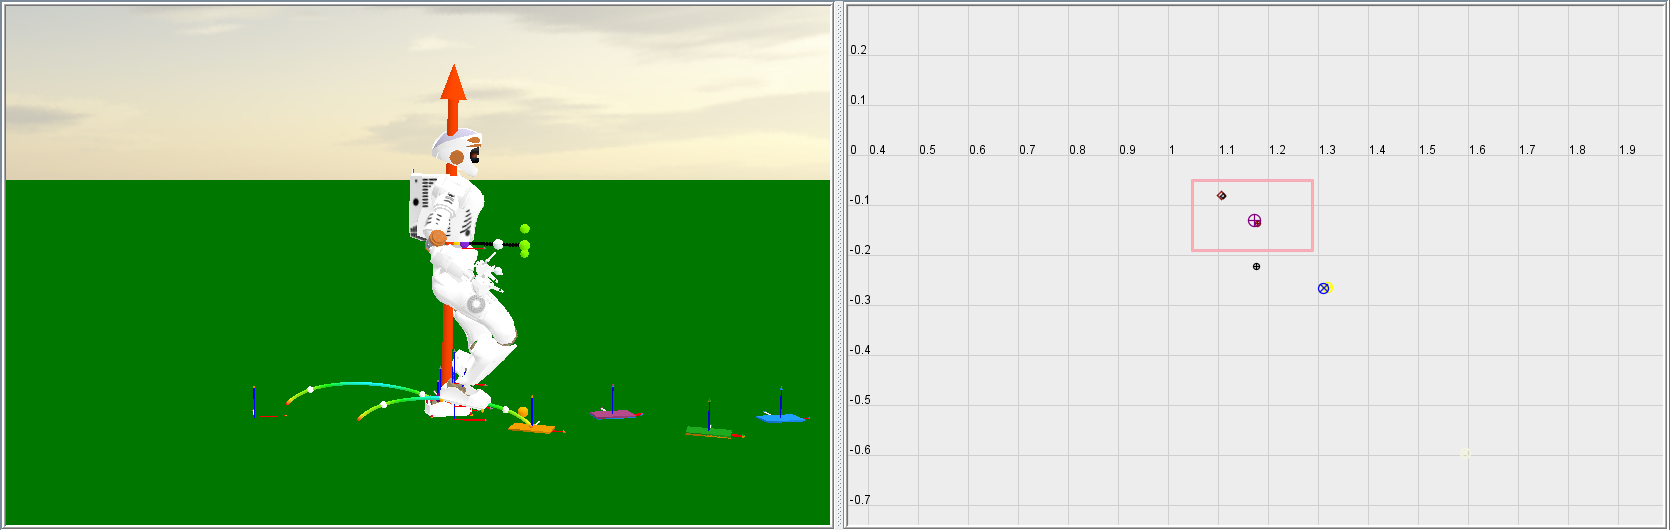
\includegraphics[width=0.8\textwidth]{STYLESTUFF/SCSValSS.png}
\caption{Valkyrie walking in \ac{SCS}. In the left window a footstep plan is made visible together with the swing leg trajectories with their knot points. The red arrow indicates the ground reaction wrench and the window on the right displays the current ground contact with some reference and measured points.}
\label{fig:scsval}
\end{figure}

\section{Control}
To track a generated high level plan the system has to be controlled. PID-control, LQR and MPC are all used in humanoid robotics. Again, there are differences in joint-level control and for example the control of the desired \ac{CoM} position, which often are separated in high level and low level control. In some cases, like with the \ac{HZD} approach as described in \cite{westervelt2003hybrid}, there is no decoupling between such levels. However, the \ac{HZD} is for this reason often applied to simpler robots, as in the mentioned paper and on ATRIAS. Furthermore, the \ac{HZD} approach is designed for systems with a degree of underactuation of one, which corresponds more to a \ac{2D} than a \ac{3D} robot model. 
\subsection{High level control}
Tracking the \ac{ICP} trajectory as is done at IHMC is an example of high level control. The robot in this stage can be seen as a \ac{LIP} with a finite sized foot and body angular momentum. At a current footstep, using the right combination of ankle torque and angular momentum, the robots motion can in theory be controlled considering the simplified \ac{LIP} model. The robot is assumed to keep itself at a constant height and expected to generate the desired centroidal momentum. Simplification of the model to only a \ac{CoM}, angular momentum and a ground reaction force, makes control more accessible than looking at joint level. The desired values of the high level controller are send to a mid level controller to translate this information to joint level control.
\subsection{Mid and low level control}
As the real robot is not a \ac{LIP} and cannot generate high level control inputs as angular momentum as a single control input, other layers of control are needed: mid and low level control. Low level controllers are often based on inverse kinematics and inverse dynamics. This concept is also widely used in industrial robotic manipulators, as for example in \cite{asada1990inverse}. What often the basis is for desired motions on joint scale is the fact that so called centroidal dynamics about the pelvis or \ac{CoM} have to equal the wrenches applied on the environment, as for example in \cite{kajita2003resolved} and \cite{koolen2016design}. An important constraint on wrenches applicable on the environment is the unilaterality of the contact and the available contact friction. This is often captured in having a so called wrench cone above the foot, wherein the resulting ground wrench has to lie. The centroidal dynamics are a combination of the linear and angular momentum rate. In \figref{fig:controlframework} an overview of the controller structure at IHMC is given. The momentum rate of change objective consist during walking mainly of the linear momentum rate as in Eq. \eqref{eq:ldot}. The motion tasks are for example moving the swing leg. This information from the high level controller is then translated in a quadratic program, that defines the solution as a set of joint accelerations and reaction wrenches. This is translated to joint level with inverse dynamics.
\begin{figure}[h]
\centering
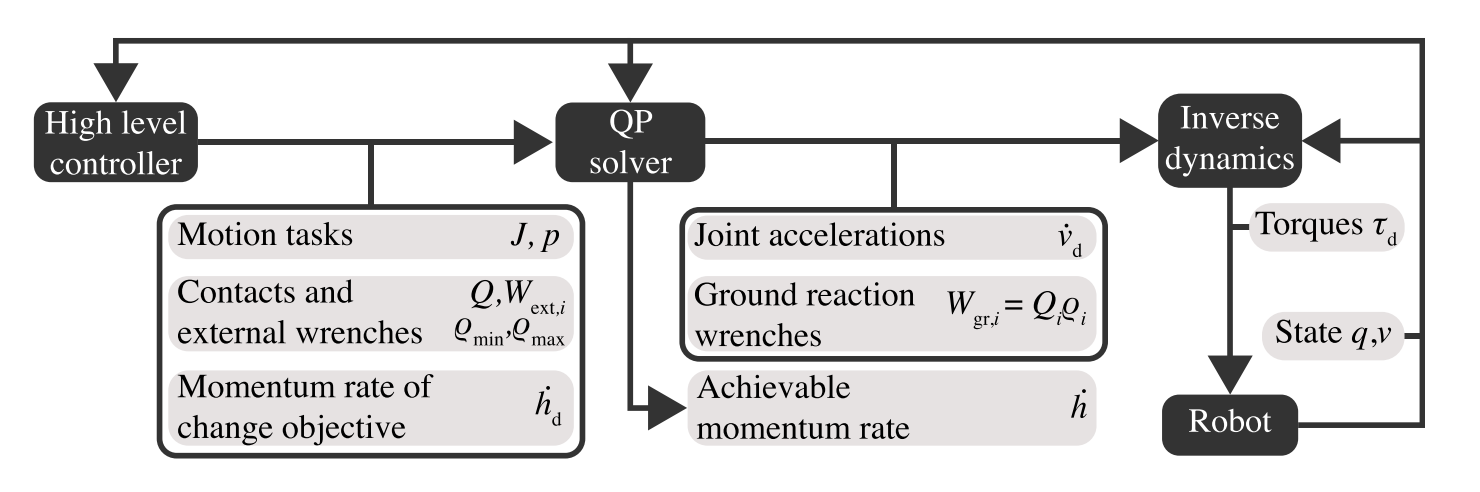
\includegraphics[width=0.8\textwidth]{STYLESTUFF/controlframework.png}
\caption{Overview of control framework used at IHMC, retrieved from \cite{koolen2016design}}
\label{fig:controlframework}
\end{figure}
\subsection{Compliant control}
In the walking of a bipedal robot with legs hybrid switching between swing and stance, a problem gets introduced with this hybrid phase shift. During swing, a trajectory is tracked using a control strategy that links more to position tracking. When the foot hits the ground, it switches instantly to the stance phase, where its position is fixed and its control actions are mainly based on forces. This instant switch can cause instabilities in the controller and an agile, compliant control strategy is needed. In \cite{sentis2006whole} is described how for different phases a different set of controller gains can be used to deal with the difference of impedance needed in control. 

\section{State Estimation} 
As state estimation is dependent on the available sensor data and the quality of the data, the possible strategies for estimation depend on the particular robot model. Typically, the robot has position sensing in all joints, that sometimes have torque sensing as well. An \ac{IMU} can be present in the body, or even in some body parts. State estimation of for example the pelvis orientation and velocity can be done by combining sensor data from both the body \ac{IMU} and an inverse dynamics algorithm that uses information from joints. On joint level, a low-pass filter can be applied and then based on the dynamics of the robot, a heuristic approach in combining the \ac{IMU} and joint data can be used to estimate the pelvis state, as is done in \cite{koolen2016design}. Another possibility is the use of more sophisticated sensor fusing techniques as the \ac{EKF}, as in \cite{kuindersma2016optimization}. Due to the complexity of the system this can be however challenging, especially with application on hardware. 

\section{Analysis \& Discussion}
The entire framework to plan and control the motion of a humanoid robot is so extensive, that it is important to narrow the areas of focus. The knowledge gained from the investigation for this chapter gives a good basis of understanding what the current bottle necks in humanoid robot control and planning are. The current frameworks do not regard any height variation of the inverted pendulum model most of the times, which of course is not done without reasons. First, a linearized model is very desirable in control, as the computational cost of such is much lower than with nonlinear ones. Second, with the linear model a plan through the \ac{3D} world can by dynamics mostly captured in a \ac{2D} plan, which simplifies the planning problem a lot. \\
For a varying height model the computation time might be an important aspect, especially for control and online planning, as full pendulum or robot dynamics are nonlinear. This has to be taken into consideration. 